\section{Benchmarking the JVM}
\label{sec:bench:jvm}

The rationale behind this section is best introduced with a warning
from Computer Architecture: A Quantitative Approach \cite{Hennessy02}
p. 63:

\begin{quote}
Virtually every practicing computer architect knows Amdahl�s Law.
Despite this, we almost all occasionally fall into the trap of
expending tremendous effort optimizing some aspect of a system
before we measure its usage. Only when the overall speedup is
unrewarding do we recall that we should have measured the usage of
that feature before we spent so much effort enhancing it!
\end{quote}
%
We measured how Java programs use the bytecode instruction set and
explored the typical and worst-case method sizes. Our measurements
and other reports are presented in the following sections.

\subsection{Bytecode Frequency}

The dynamic instruction frequency is the main measurement for
determining a processor implementation. We can identify those
instructions that should be fast. For seldom-used instructions, a
trade-off can be made between performance and hardware resources.

Many reports have been written about JVM bytecode frequencies (e.g.\
\cite{Greg2002, 365338, 624084}). Most of these reports provide only
a coarse categorization of the bytecodes. For example, the bytecodes
\code{iload\_n} (load an \code{int} from a local variable) and
\code{getfield} (fetch a field from an object) are combined in one
instruction category. However, these instructions are very different
in terms of their implementation complexity. We have chosen a
fine-grained categorization of the bytecodes to gain greater insight
into the bytecode usage. In Table~\ref{tab_java_instr_cat} all 201
bytecode instructions are listed by category.


\begin{table}
    \centering
    \begin{tabular}{ll}
    \toprule
    Type & Bytecode \\
    \midrule

    load
    & aload, dload, fload, iload, lload \\

    load (short)
    & aload\_0, aload\_1, aload\_2, aload\_3, \\
    & dload\_0, dload\_1, dload\_2, dload\_3, \\
    & fload\_0, fload\_1, fload\_2, fload\_3, \\
    & iload\_0, iload\_1, iload\_2, iload\_3, \\
    & lload\_0, lload\_1, lload\_2, lload\_3 \\

    store
    & astore, dstore, fstore, istore, lstore \\

    store (short)
    & astore\_0, astore\_1, astore\_2, astore\_3, \\
    & dstore\_0, dstore\_1, dstore\_2, dstore\_3, \\
    & fstore\_0, fstore\_1, fstore\_2, fstore\_3, \\
    & istore\_0, istore\_1, istore\_2, istore\_3, \\
    & lstore\_0, lstore\_1, lstore\_2, lstore\_3 \\

    const
    & bipush, ldc, ldc\_w, ldc2\_w, sipush \\

    const (short)
    & aconst\_null, dconst\_0, dconst\_1, fconst\_0, fconst\_1, fconst\_2, \\
    & iconst\_0, iconst\_1, iconst\_2, iconst\_3, iconst\_4, iconst\_5, \\
    & iconst\_m1, lconst\_0, lconst\_1 \\

    get
    & getfield, getstatic \\

    put
    & putfield, putstatic \\

    alu
    & dadd, ddiv, dmul, dneg, drem, dsub, \\
    & fadd, fdiv, fmul, fneg, frem, fsub, \\
    & iadd, iand, idiv, imul, ineg, ior, irem, ishl, ishr, isub, iushr, ixor, \\
    & ladd, land, ldiv, lmul, lneg, lor, lrem, lshl, lshr, lsub, lushr, lxor \\

    iinc
    & iinc \\

    stack
    & dup, dup\_x1, dup\_x2, dup2, dup2\_x1, dup2\_x2, pop, pop2, swap \\

    array
    & aaload, aastore, baload, bastore, caload, castore, daload, dastore, \\
    & faload, fastore, iaload, iastore, laload, lastore, saload, sastore \\

    branch
    & goto, goto\_w, if\_acmpeq, if\_acmpne, if\_icmpeq, \\
    & if\_icmpge, if\_icmpgt, if\_icmple, if\_icmplt, if\_icmpne, \\
    & ifeq, ifge, ifgt, ifle, iflt, ifne, ifnonnull, ifnull \\

    compare
    & dcmpg, dcmpl, fcmpg, fcmpl, lcmp \\

    switch
    & lookupswitch, tableswitch \\

    call
    & invokeinterface, invokespecial, invokestatic, invokevirtual \\

    return
    & areturn, dreturn, freturn, ireturn, lreturn, return \\

    conversion
    & d2f, d2i, d2l, f2d, f2i, f2l, i2b, i2c, i2d, i2f, i2l, i2s, l2d, l2f, l2i \\

    new
    & anewarray, multianewarray, new, newarray \\

    other
    & arraylength, athrow, checkcast, instanceof, jsr, jsr\_w, \\
    & monitorenter, monitorexit, nop, ret, wide \\


    \bottomrule
    \end{tabular}
    \caption[Categories of JVM bytecodes]{The 201 Java bytecodes and
    their assignment to different categories}
    \label{tab_java_instr_cat}
\end{table}


Three different applications were run on an instrumented JVM to
measure dynamic bytecode frequency. The results were compared with
the results from the above-mentioned reports. In
Table~\ref{tab_java_instr_frequ} the dynamic instruction count for
the three different benchmarks is shown. The last column is the
average of the three tests weighted by the individual instructions
count.

Kaffe \cite{kaffe} is an independent implementation of the JVM
distributed under the GNU Public License. Kaffe was instrumented to
collect data on dynamic bytecode usage. Three different applications
were used as benchmarks to obtain the dynamic instruction count:
JLex, KCJ and javac. JLex \cite{jlex} is a lexical analyzer
generator, written for Java in Java. The data was collected by
running JLex with the provided \code{sample.lex} as the input file.
KJC \cite{kcj} is a Java compiler in Java, freely available under the
terms of the GNU General Public License. javac is the Sun Java
compiler. Both compilers were compiling part of the KJC sources
during the benchmark. These benchmarks are similar to the benchmarks
used in other reports and the results are therefore comparable.
However, typical embedded applications can result in a slightly
different instruction set usage pattern. Embedded applications are
usually tightly connected with the environment and are therefore not
available as stand-alone programs to serve as benchmarks. An embedded
application developed on JOP was adapted to serve as a benchmark for
Section~\ref{sec:cache} and Chapter~\ref{chap:results}.

%19,572,165 + 951,138,375 + 341,926,231 = 1,312,636,771

% JLex.Main   kaffe JLex.Main JLex/sample.lex
% at.dms.kjc.Main:
%    kaffe -cp kjc-2.1B-bin.jar at.dms.kjc.Main -d classes kopi-2.1B/src/kjc/*.java
% com.sun.tools.javac.Main:
%    kaffe -cp /usr/lib/java/lib/tools.jar com.sun.tools.javac.Main -d classes kopi-2.1B/src/kjc/*.java
%  stops with compile error


\begin{table}
    \centering
    \begin{tabular}{lrrrr}
        \toprule
        & JLex & KJC & javac & Average \\
        \midrule
        load (short) & 32.72 & 31.45 & 27.24 & 30.37 \\
        get & 12.02 & 14.39 & 17.04 & 15.04 \\
        branch & 11.26 & 10.40 & 10.71 & 10.49 \\
        invoke & 6.87 & 6.31 & 4.24 & 5.77 \\
        return & 6.82 & 6.20 & 4.17 & 5.68 \\
        load & 7.59 & 4.19 & 7.48 & 5.09 \\
        alu & 2.60 & 4.43 & 4.74 & 4.48 \\
        const (short) & 4.61 & 4.26 & 4.74 & 4.39 \\
        array & 4.22 & 4.07 & 3.22 & 3.85 \\
        put & 0.78 & 2.14 & 3.65 & 2.52 \\
        iinc & 1.81 & 2.38 & 1.41 & 2.12 \\
        stack & 1.30 & 2.11 & 2.11 & 2.10 \\
        store (short) & 2.61 & 2.18 & 1.71 & 2.06 \\
        other & 1.63 & 2.22 & 1.21 & 1.95 \\
        const & 0.85 & 1.56 & 2.80 & 1.87 \\
        store & 2.05 & 0.85 & 1.94 & 1.15 \\
        conversion & 0.02 & 0.36 & 0.58 & 0.42 \\
        switch & 0.00 & 0.20 & 0.60 & 0.30 \\
        new & 0.08 & 0.28 & 0.20 & 0.25 \\
        compare & 0.14 & 0.03 & 0.22 & 0.08 \\
        \bottomrule
    \end{tabular}
    \caption{Dynamic bytecode frequency in \%}
    \label{tab_java_instr_frequ}
\end{table}

\begin{table}
    \centering
    \begin{tabular}{lrlr}
        \toprule
        \multicolumn{2}{c}{JLex, KJC and javac} &
        \multicolumn{2}{c}{SPEC and Java Grande} \\
        \cmidrule(lr){1-2} \cmidrule(lr){3-4}
        Instruction & Frequency & Instruction & Frequency \\
        \midrule
        load (short)  & 30.37 & acnst &  0.07 \\
        load          &  5.09 & aload & 16.23 \\
        const (short) &  4.39 & fcnst &  0.33 \\
        const         &  1.87 & fload &  6.33 \\
                      &       & icnst &  3.21 \\
                      &       & iload & 18.06 \\
        \midrule
        load \& const & \textbf{41.72}& & \textbf{44.77} \\
        \midrule
        get           & 15.04 & field & 11.12 \\
        put           &  2.52 &       &       \\
        \midrule
        field access & \textbf{17.56} & & \textbf{11.12} \\
        \midrule
        branch        & 10.49 & cjump &  5.67 \\
        compare       &  0.08 & ujump &  0.51 \\
        \midrule
        control & \textbf{10.57}& & \textbf{6.18} \\
        \midrule
        invoke & \textbf{5.77} & fcall &  \textbf{3.63} \\
        \midrule
        return &  \textbf{5.68} & retrn &  \textbf{2.07} \\
        \bottomrule
    \end{tabular}
    \caption[Dynamic bytecode frequency comared]
    {Dynamic bytecode frequency compared with the
    measurements from \cite{Dowling2002}}
    \label{tab:java:instr:frequ:comp}
\end{table}

In \cite{Dowling2002} the relationship between static and dynamic
instruction frequency of 19 programs from the SPECjvm98
\cite{SPECJvm98} and Java Grande benchmark suites were measured. The
bytecodes categories were chosen differently from the above
measurements, but detailed enough to verify our own measurements.
\tablename~\ref{tab:java:instr:frequ:comp} shows the average dynamic
execution frequency in percent\footnote{The values do not add up to
100\% as only the most significant bytecode categories are shown} of
selected bytecode categories from the SPEC and Java Grande
benchmarks, compared with the results obtained by our measurements.
The numbers in bold are categories or sums of categories that are
comparable. The frequency of the ``load \& const" instructions is
very similar to that in our measurements. However, field access,
control instructions and method invocations are more frequent in our
measurements. The higher count on field access instructions and
method invocation can result from a more object oriented programming
style in our selected applications than in the SPEC and Java Grande
benchmarks. The big difference, not seen in our measurements, between
the invoke and return frequency in the SPEC and Java Grande
benchmarks is not explained in \cite{Dowling2002}.

In all measurements, the load of local variables and constants onto
the stack accounts for more than 40\% of instructions executed. This
feature shows that an efficient realization of the local variable
memory area, the stack and the transfer between these memory areas
is mandatory.

The next most executed bytecodes (\code{getfield} and
\code{getstatic}) are the instructions that load an object or class
field onto the operand stack. To account for these frequent
instructions, the class layout for the runtime system has to be
optimized for quick resolution of field addresses (i.e.\ minimum
memory indirections).

The frequency of branches is comparable with the SPECint2000
measurements on RISC processors \cite{Hennessy02}. With such a high
branch frequency, a processor without branch prediction logic is put
under pressure in terms of pipeline length.

It is interesting to note that there are more method invoke
instructions than return instructions. Two facts are responsible for
this difference: native methods are invoked by a bytecode, but the
return is inside the native methods; and an exception can result in
a method exit without return.


\subsection{Methods Types and Length}
\label{sec:bench:jvm:methods}

\tablename~\ref{tab_java_meth_type} shows the number of dynamic
method calls of the Java Grande and \linebreak[4]SPECjvm98
benchmarks. It can be seen that the distribution of method types
depends on the application type. Usage of virtual methods and
interfaces is common in OO programming. Static methods result from
the simple translation of procedural programs to Java.

\begin{table}
    \centering
    \begin{tabular}{lrrrr}
        \toprule
         & virtual & special & static & interface \\
        \midrule
        Java Grande & 57.1 & 8.7 & 34.2 & 0.0 \\
        SPEC JVM98 & 81.0 & 10.9 & 2.9 & 5.2 \\
        \bottomrule
    \end{tabular}
    \caption{Types of different dynamic method calls for two benchmarks (from \cite{Power2002})}
    \label{tab_java_meth_type}
\end{table}

As a basis for the proposed cache solution in
Section~\ref{sec:cache}, we will explore static distribution of
method sizes. In the JVM, only relative branches are defined. The
conditional branches and goto have an offset of 16 bits, resulting
in a practical limit of the method length of 32KB. Although there is
a goto instruction with a wide index (\emph{goto\_w}) that takes a
4-byte branch offset, other factors (e.g.\ indices in the exception
table) limit the size of a method to 65535 bytes.

Radhakrishnan et al.\ \cite{365338} measured the dynamic method size
of the SPEC suite. They observed a `tri-nodal' distribution, where
most of the methods were 1, 9, or 26 bytecodes long. No explanation
is given for the sizes of 9 or 26. The explanation of the 1 bytecode
long methods as \emph{wrapper methods} is wrong. For a wrapper
method, the method needs to contain a minimum of two instructions (an
invoke and a return). A single instruction method can \emph{only}
contain a return. However, this observation is in sharp contrast to
the measurements obtained by Power and Waldron in \cite{Power2002}.




\begin{table}
    \centering
    \begin{tabular}{rrrr}
        \toprule
        Length & Methods & Percentage & Cumulative \\
        & & & percentage \\
        \midrule
        1 & 1,388 & 1.94 & 1.94 \\
        2 & 1,580 & 2.21 & 4.16 \\
        4 & 1,871 & 2.62 & 6.78 \\
        8 & 16,192 & 22.67 & 29.45 \\
        16 & 12,363 & 17.31 & 46.76 \\
        32 & 12,638 & 17.70 & 64.45 \\
        64 & 11,178 & 15.65 & 80.10 \\
        128 & 7,287 & 10.20 & 90.31 \\
        256 & 4,304 & 6.03 & 96.33\\
        512 & 1,727 & 2.42 & 98.75 \\
        1,024 & 592 & 0.83 & 99.58 \\
        2,048 & 175 & 0.25 & 99.83 \\
        4,096 & 75 & 0.11 & 99.93 \\
        8,192 & 37 & 0.05 & 99.98 \\
        16,384 & 11 & 0.02 & 100.00 \\
        32,768 & 1 & 0.00 & 100.00 \\
        65,536 & 0 & 0.00 & 100.00 \\
        \bottomrule
    \end{tabular}
    \caption{Static method count of different sizes from the runtime library (JDK 1.4).}
    \label{tab_java_jdk_static_size}
\end{table}

In Table~\ref{tab_java_jdk_static_size}, the number of methods of
different sizes in the Java runtime library (JDK 1.4) is shown. The
library consists of 71419 methods, the largest being 16706 bytes.
The size is classified by powers of 2 because we are interested in
the size of cache memory for complete methods. In the table, the row
of, for example, size 32 includes all methods of a size from 17 to
32 bytes. It can be seen that methods are typically very short. In
fact, 99\% of the methods are less than 513 bytes in size. This
property is important for the proposed method cache in
Section~\ref{sec:cache}, where a complete method has to fit into the
instruction cache.

All larger methods are different kinds of initialization functions,
in most cases \code{$<$clinit$>$()}\footnote{The class or interface
initialization method is static and the special name
\codefoot{$<$clinit$>$} is supplied by the compiler. These
initialization methods are invoked implicitly by the JVM. The
definition when these methods get invoked is problematic for the
WCET analysis (see Section~\ref{para:restrict:clinit}).}. The large
class initialization methods typically result from the
initialization of arrays with constant data. This is necessary
because of the lack of initialized data segments, such as the BSS in
C, in the Java class file. These initialization methods contain
straight-line code and can therefore be split to smaller methods
automatically, if necessary.

\begin{figure}
    \centering
    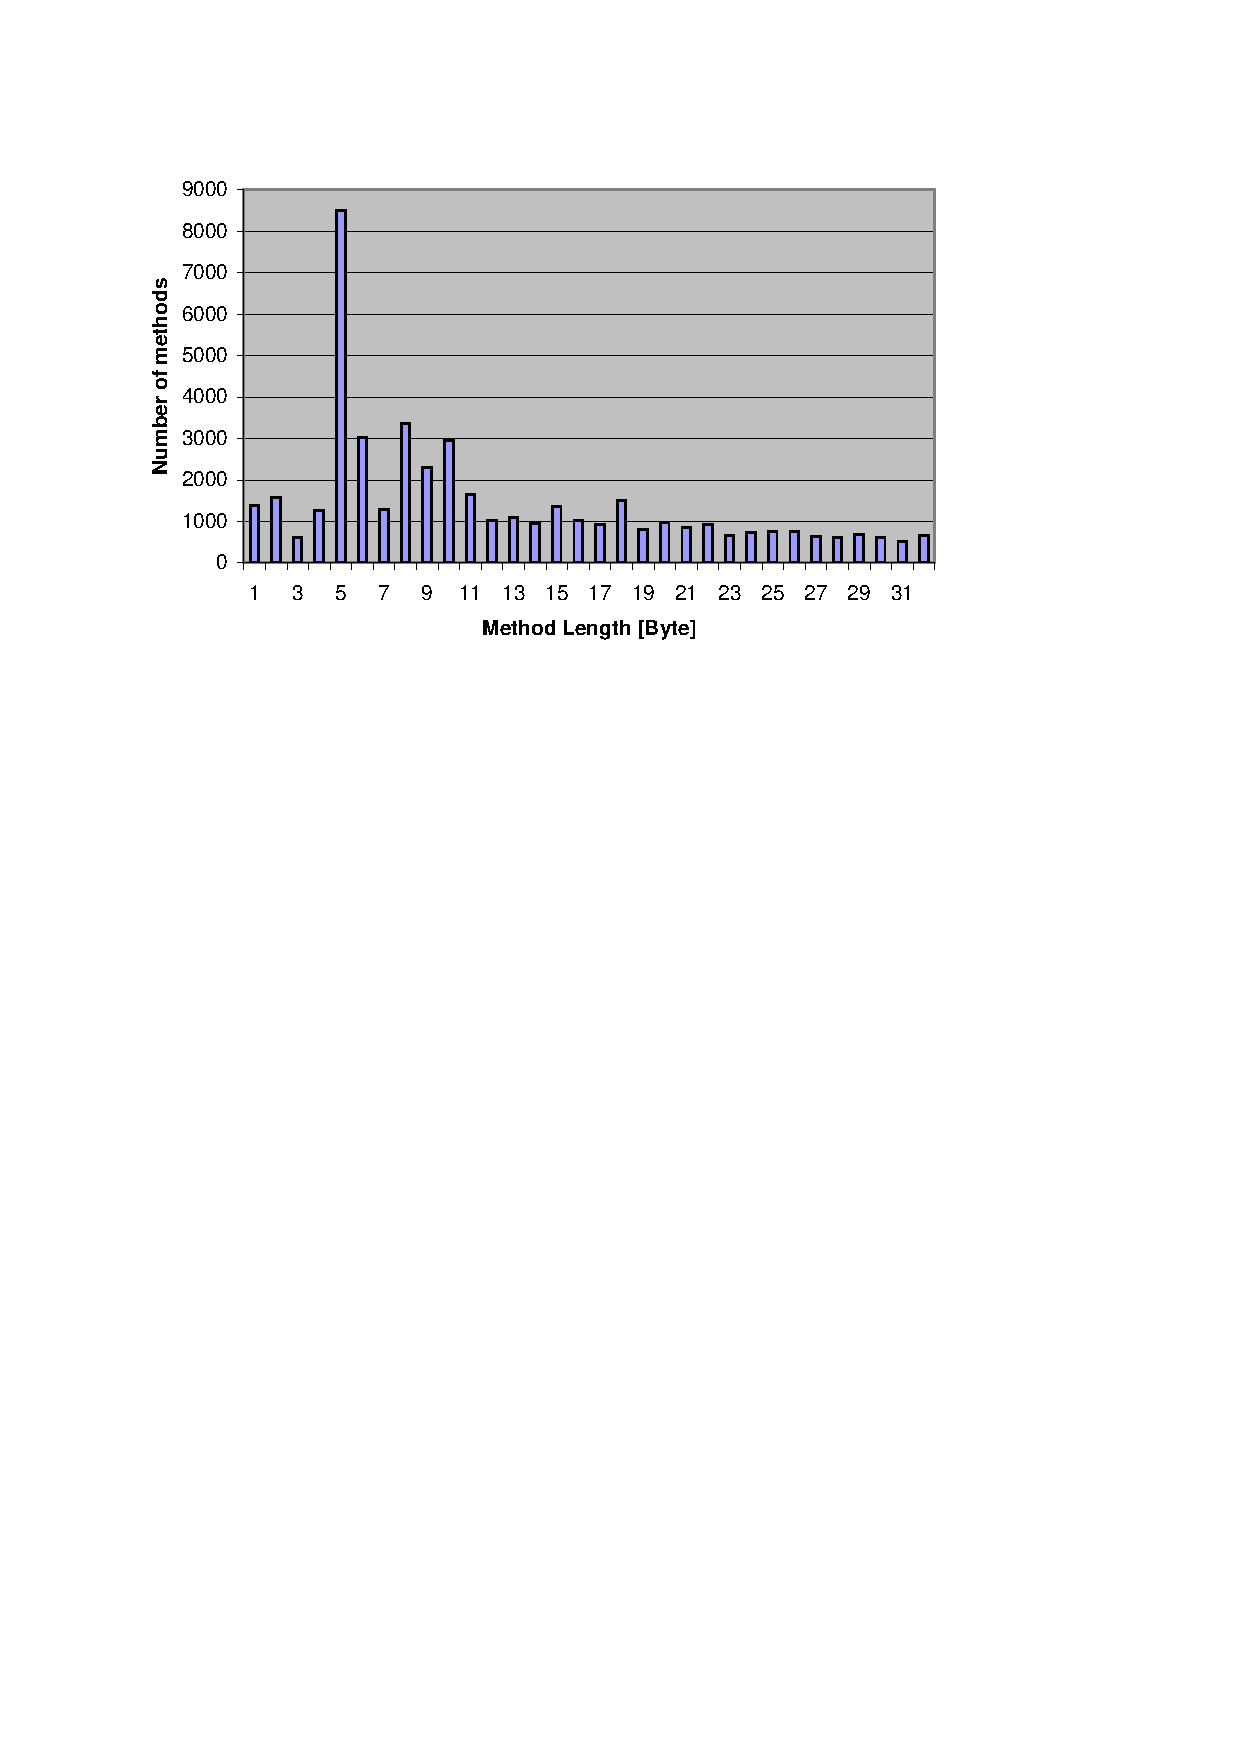
\includegraphics[width=\excelwidth]{arch/arch_meth32}
    \caption[Static method count for methods of size up to 32 bytes]
    {Static method count for methods of size up to 32 bytes in the JDK 1.4 runtime library.
    The horizontal axis indicates the method size.}
    \label{fig_java_meth32}
\end{figure}

\begin{figure}
    \centering
    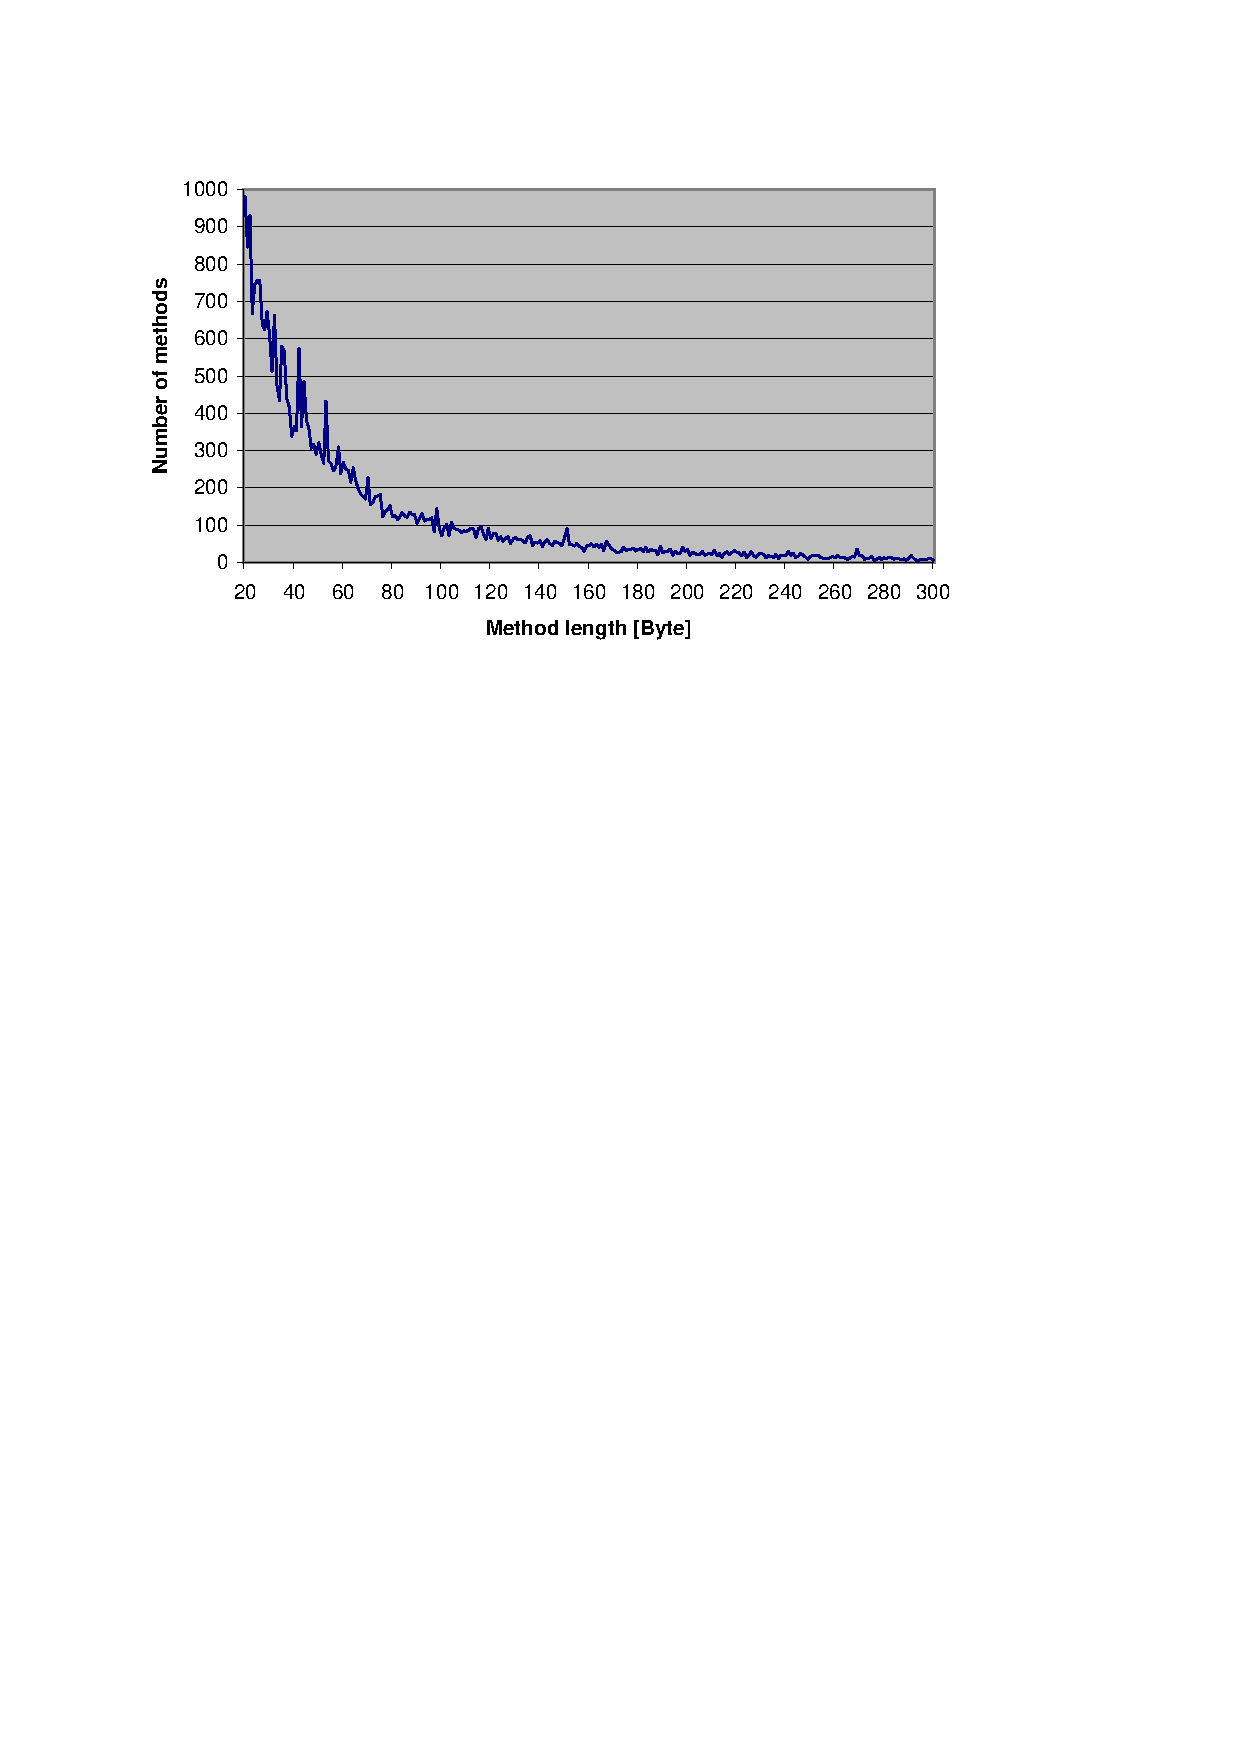
\includegraphics[width=\excelwidth]{arch/arch_meth300}
    \caption[Static method count from the JDK 1.4 runtime library]
    {Static method count from the JDK 1.4 runtime library.
    The horizontal axis indicates the method size in bytes.}
    \label{fig_java_meth300}
\end{figure}

In Figure~\ref{fig_java_meth32}, the distribution of small methods
up to a size of 32 bytes is shown.
\figurename~\ref{fig_java_meth300} shows the method count for
methods up to 300 bytes. As expected, we see fewer methods as size
increases. We observed no surprise in the distribution, unlike the
`tri-nodal' distribution in \cite{365338}. The only method size that
is very common is 5 bytes. These methods are the typical setter and
getter methods in object-oriented programming as shown in
Listing~\ref{lst:arch:java:getval}.

\begin{lstlisting}[float, caption={Bytecodes for a getter method},label=lst:arch:java:getval]
    private int val;

    public int getVal() {
        return val;
    }

    public int getVal();
    Code:
    0:   aload_0
    1:   getfield        #2; //Field val:I
    4:   ireturn
\end{lstlisting}

The method \code{getVal()} translates to three bytecodes of 1, 3 and
1 bytes in length respectively. These methods should show up in
\cite{365338} as a peak at 3 bytecodes.

The static distribution of method sizes in an application (javac,
the Java compiler) is quite similar to the distribution in the
library. In the class file that contains the Java compiler, 98\% of
the methods are smaller than 513 bytes, and the larger methods are
class initializers.

\subsection{Summary}

In this section, we performed dynamic measurements on the JVM
instruction set. We saw that more than 40\% of the executed
instructions are local variables or constants loads onto the stack.
This high frequency of stack access calls for an efficient
implementation of the stack, as described in
Section~\ref{sec:stack}.

In addition, we have statically measured method sizes. Methods are
typically very short. 30\% of the methods are shorter than 9 bytes
and 99\% account for methods of up to 512 bytes. The maximum length
is further limited by the definition of the class file. We will use
this property in the proposed \emph{method cache} in
Section~\ref{sec:cache}.

Instruction-usage data is an important input for the design of a
processor architecture, as seen in the following sections.


%\subsection{Some more properties}
%Number of local variables per method.


%\subsubsection{Some Comments}
%
%* Clarification of the quick instructions

%* A word about javac: absolute not optimized code generations.
%Simplifies JIT, but not so good for Java processors or an
%interpreting JVM

%\dots CPI is not so easy to measure for the JVM. JVM = runtime
%infrastructure (GC, new). What is measured with JIT?
